

\section{Central tracking}

%%%%%%%%%%%%%%%%%%%%%%%%%%%%%%%%%%%%%%%%%%%%
\subsection{Silicon microstrip tracker}
%%%%%% SLIDE
\begin{frame}{\textcolor{Goldenrod}{Central Tracker}}
  \begin{overlayarea}{\textwidth}{\textheight}
    \begin{figure}[h]
      \centering
      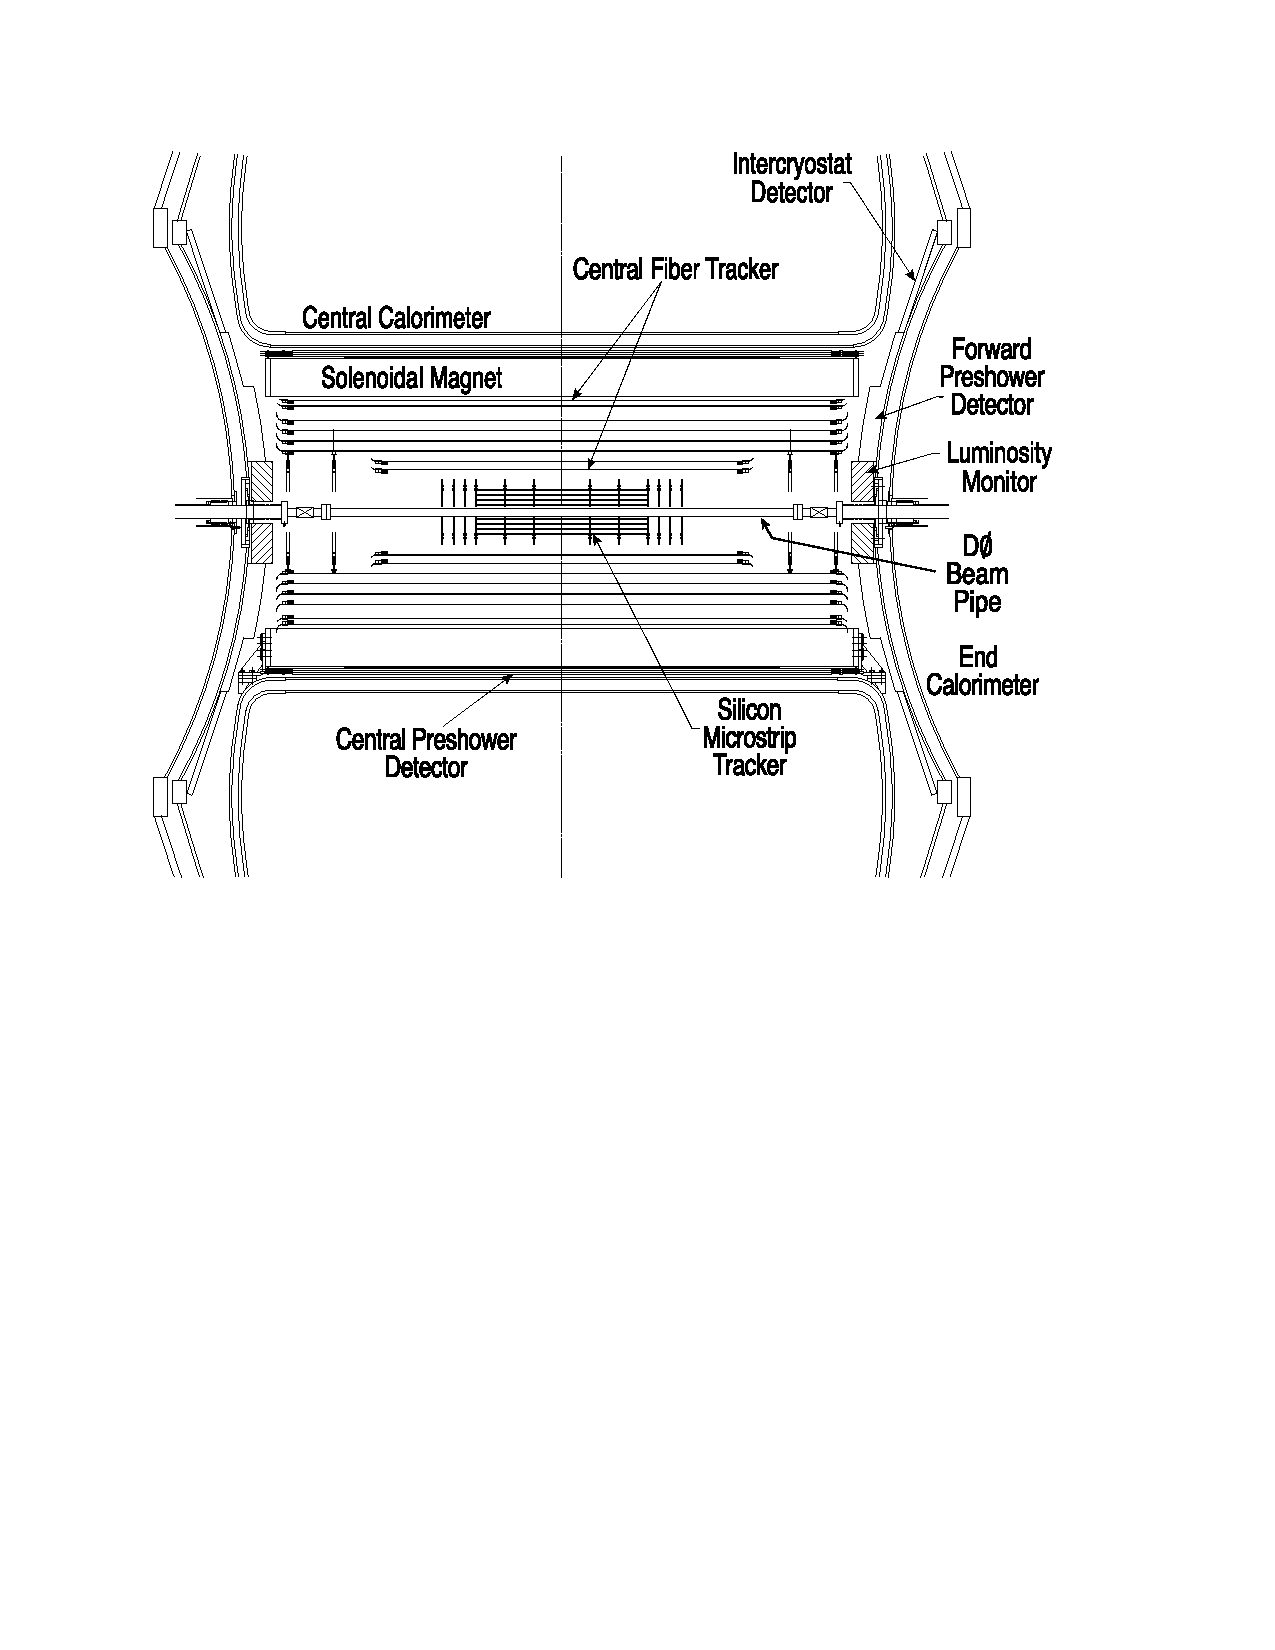
\includegraphics[height=0.4\textheight]{./Images/08_CT.pdf}
    \end{figure}
    
    \itt
  \item
    A Silicon Microstrip Tracker (SMT) and a Central Fiber Tracker
    (CFT) within a solenoidal magnet
  \item Excellent resolution; $\sigma_{d_0} \approx 15 \mu m, 
    \sigma_{z_0}\approx 35\mu m$:\\
    \hlt{Magenta}{b-tagging, good $p^{lep/jet}_{T} $ and $\slashed{E_T}$ measurement}
    \tti
  \end{overlayarea}
\end{frame}


%%%%%% SLIDE
\begin{frame}{\textcolor{Goldenrod}{Silicon Microstrip Tracker}}
  \begin{overlayarea}{\textwidth}{\textheight}
    \begin{figure}[h]\centering
      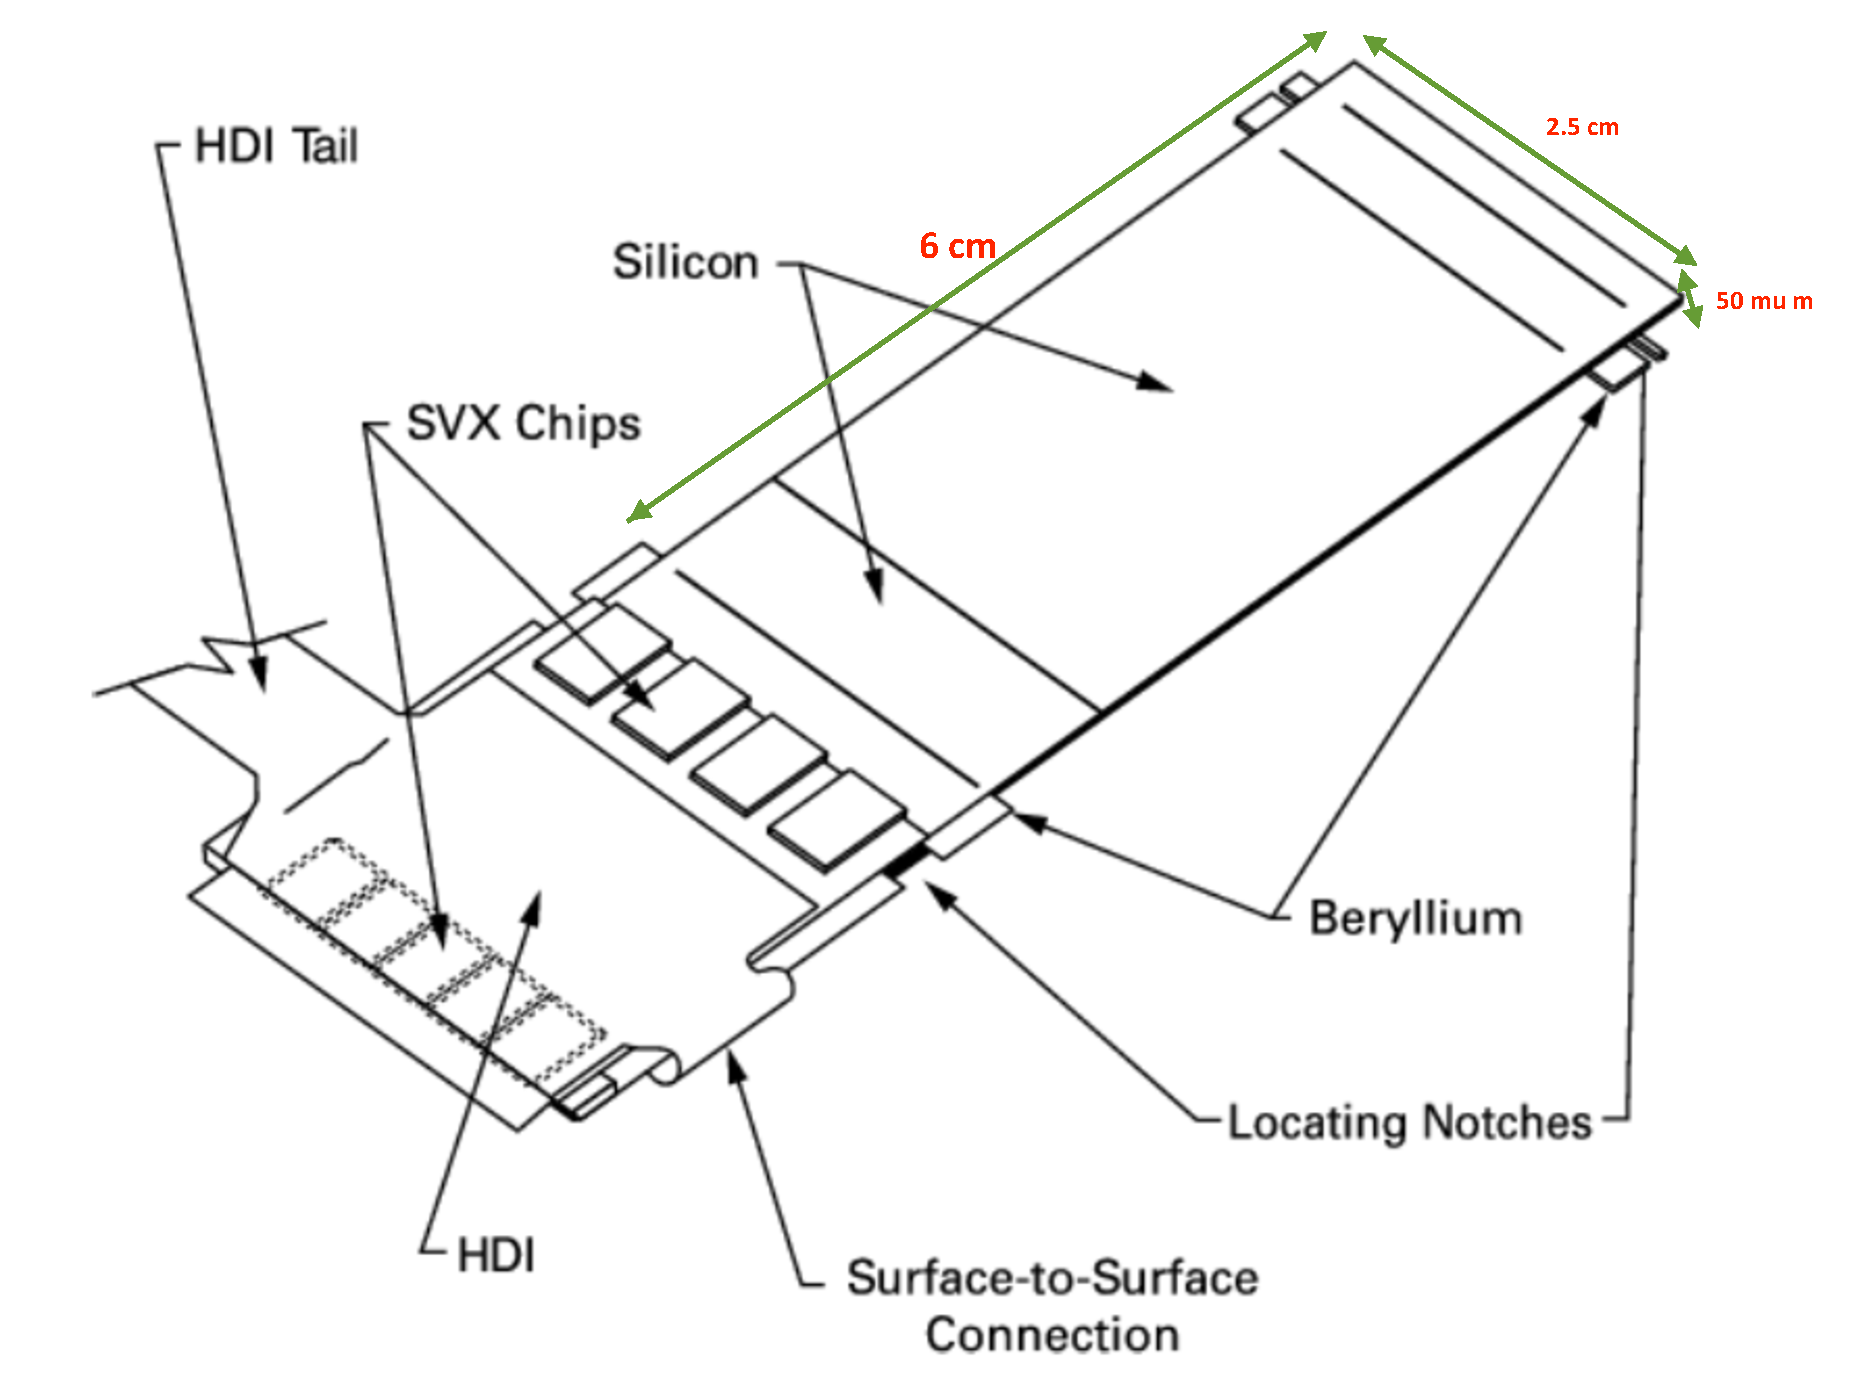
\includegraphics[height=0.3\textheight,width=0.5\textwidth]{./Images/09_SMT_03}
      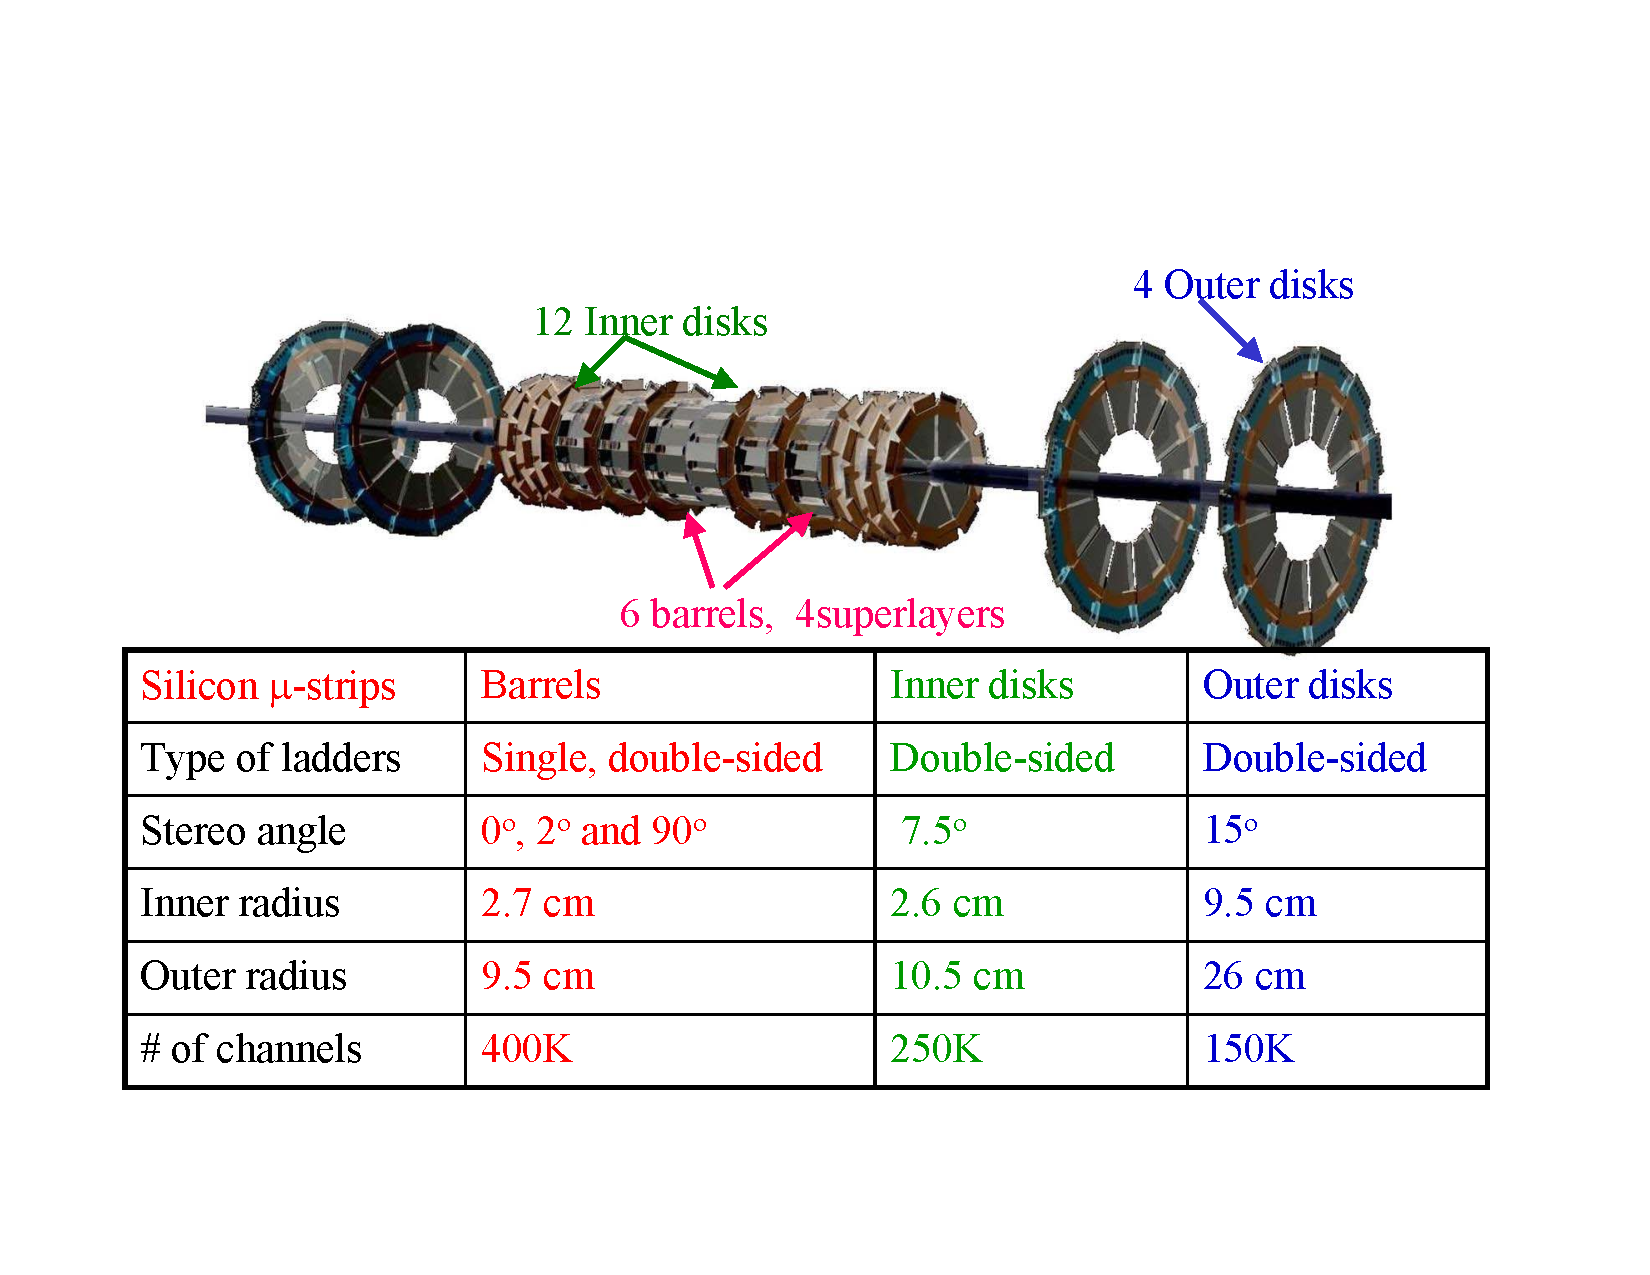
\includegraphics[height=0.3\textheight,width=0.5\textwidth]{./Images/09_SMT}
      % 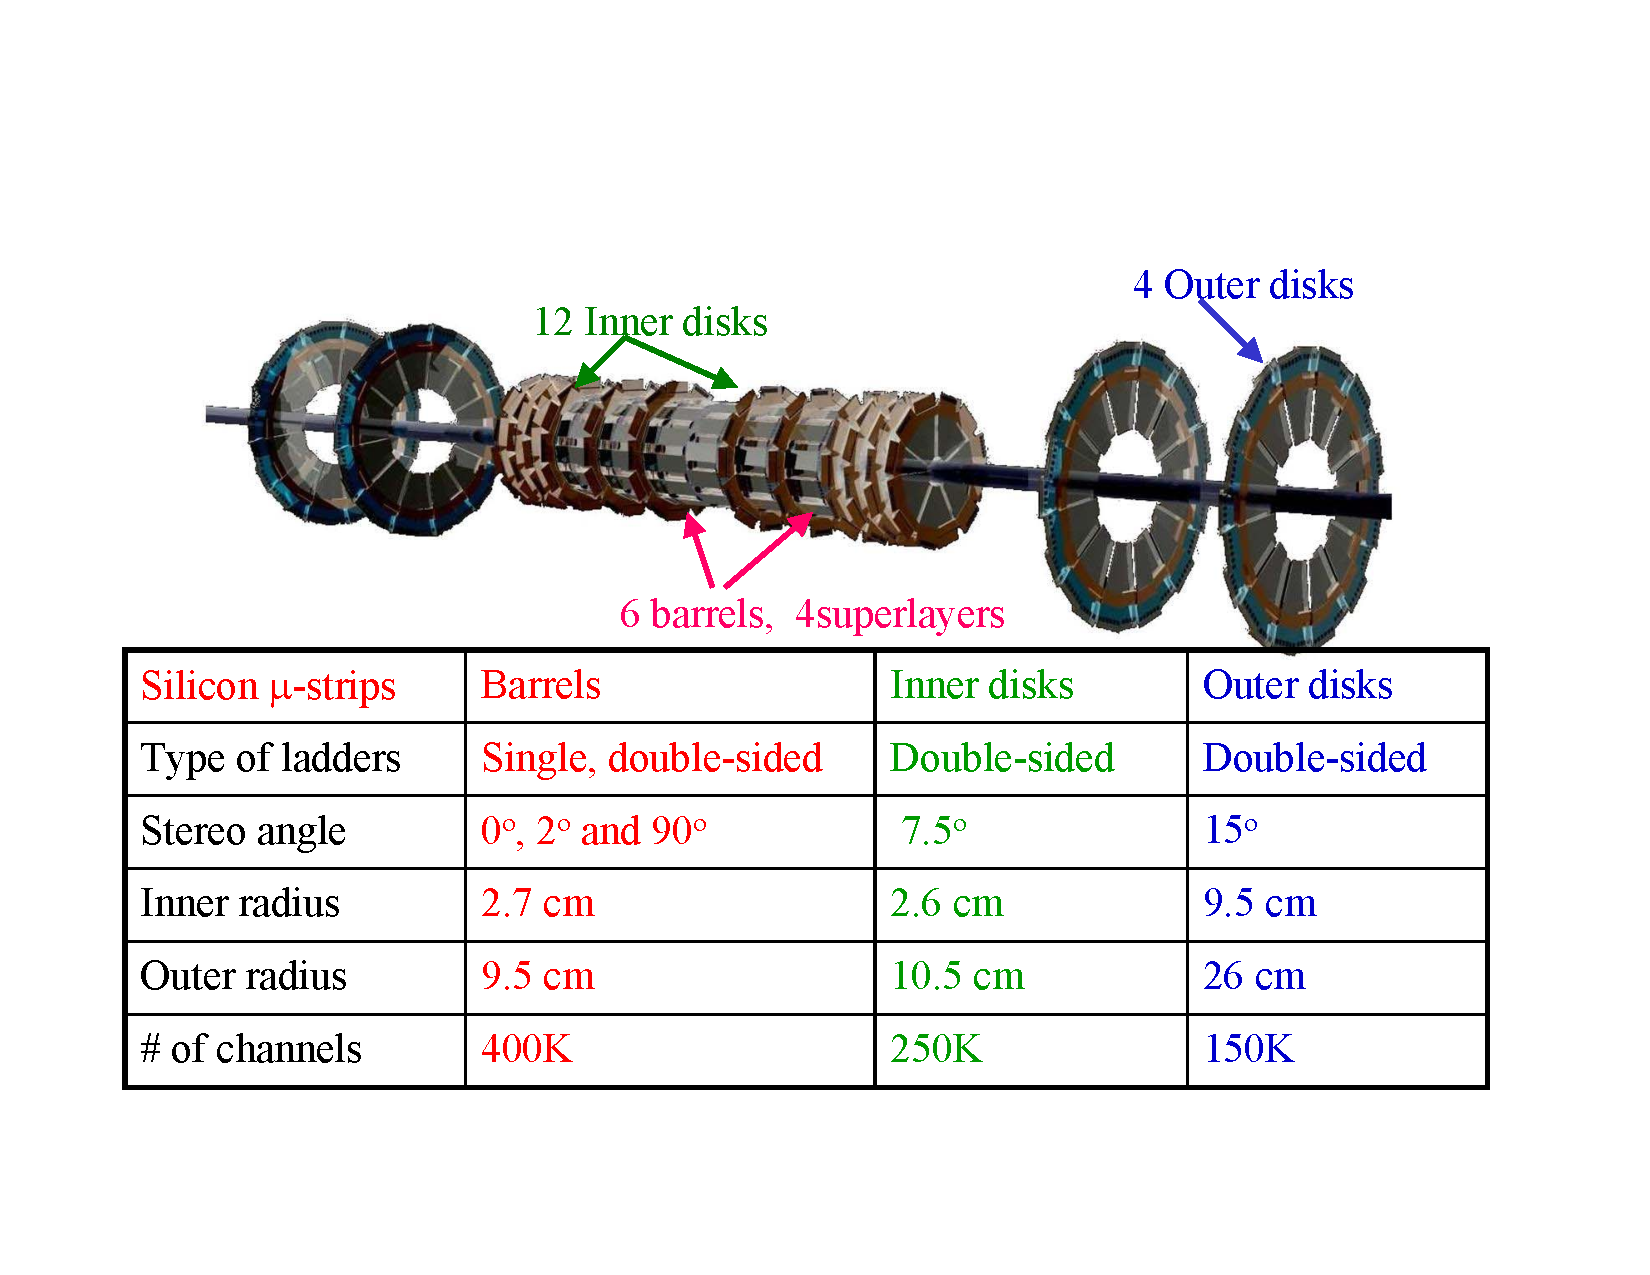
\includegraphics[height=0.3\textheight,width=0.5\textwidth]{./Images/09_SMT}
    \end{figure}
    
    \itt
  \item \hlt{black}{Design considerations:}\\ minimal mass, precise
    alignment, good thermal performance and front-end electronics.
  \item The barrel gives $(r, \phi)$ coordinate and disks give $(r,
    \phi, z)$.
  \item \hlt{Orange}{Unit cell:}\\ $1/2$
    silicon surfaces a laminated readout chip
    glued to rectangular beryllium substrates.
    \tti
\end{overlayarea}
\end{frame}
%%%%%% SLIDE
\begin{frame}{\textcolor{Goldenrod}{Silicon Microstrip Tracker}}
  \begin{overlayarea}{\textwidth}{\textheight}
    \begin{figure}[h]
      \centering
      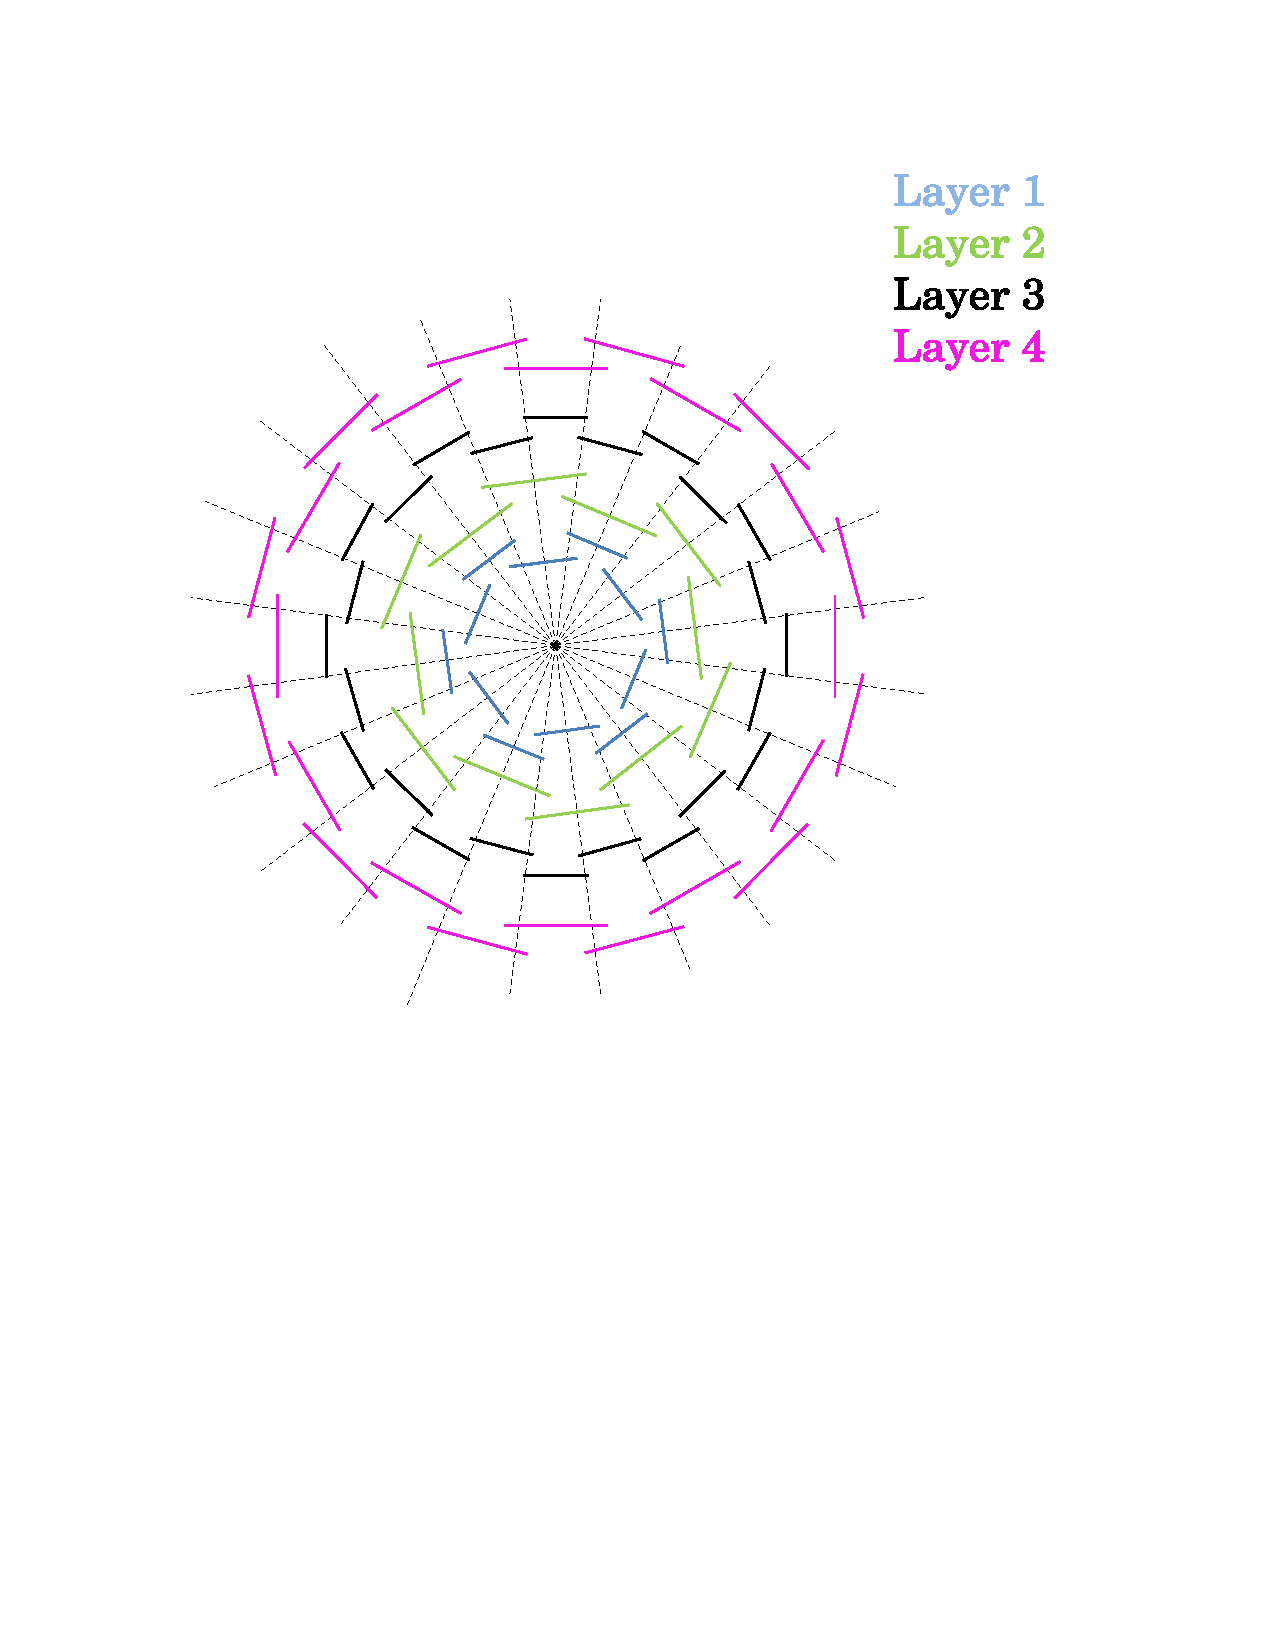
\includegraphics[height=0.6\textheight]{./Images/09_SMT_01}
      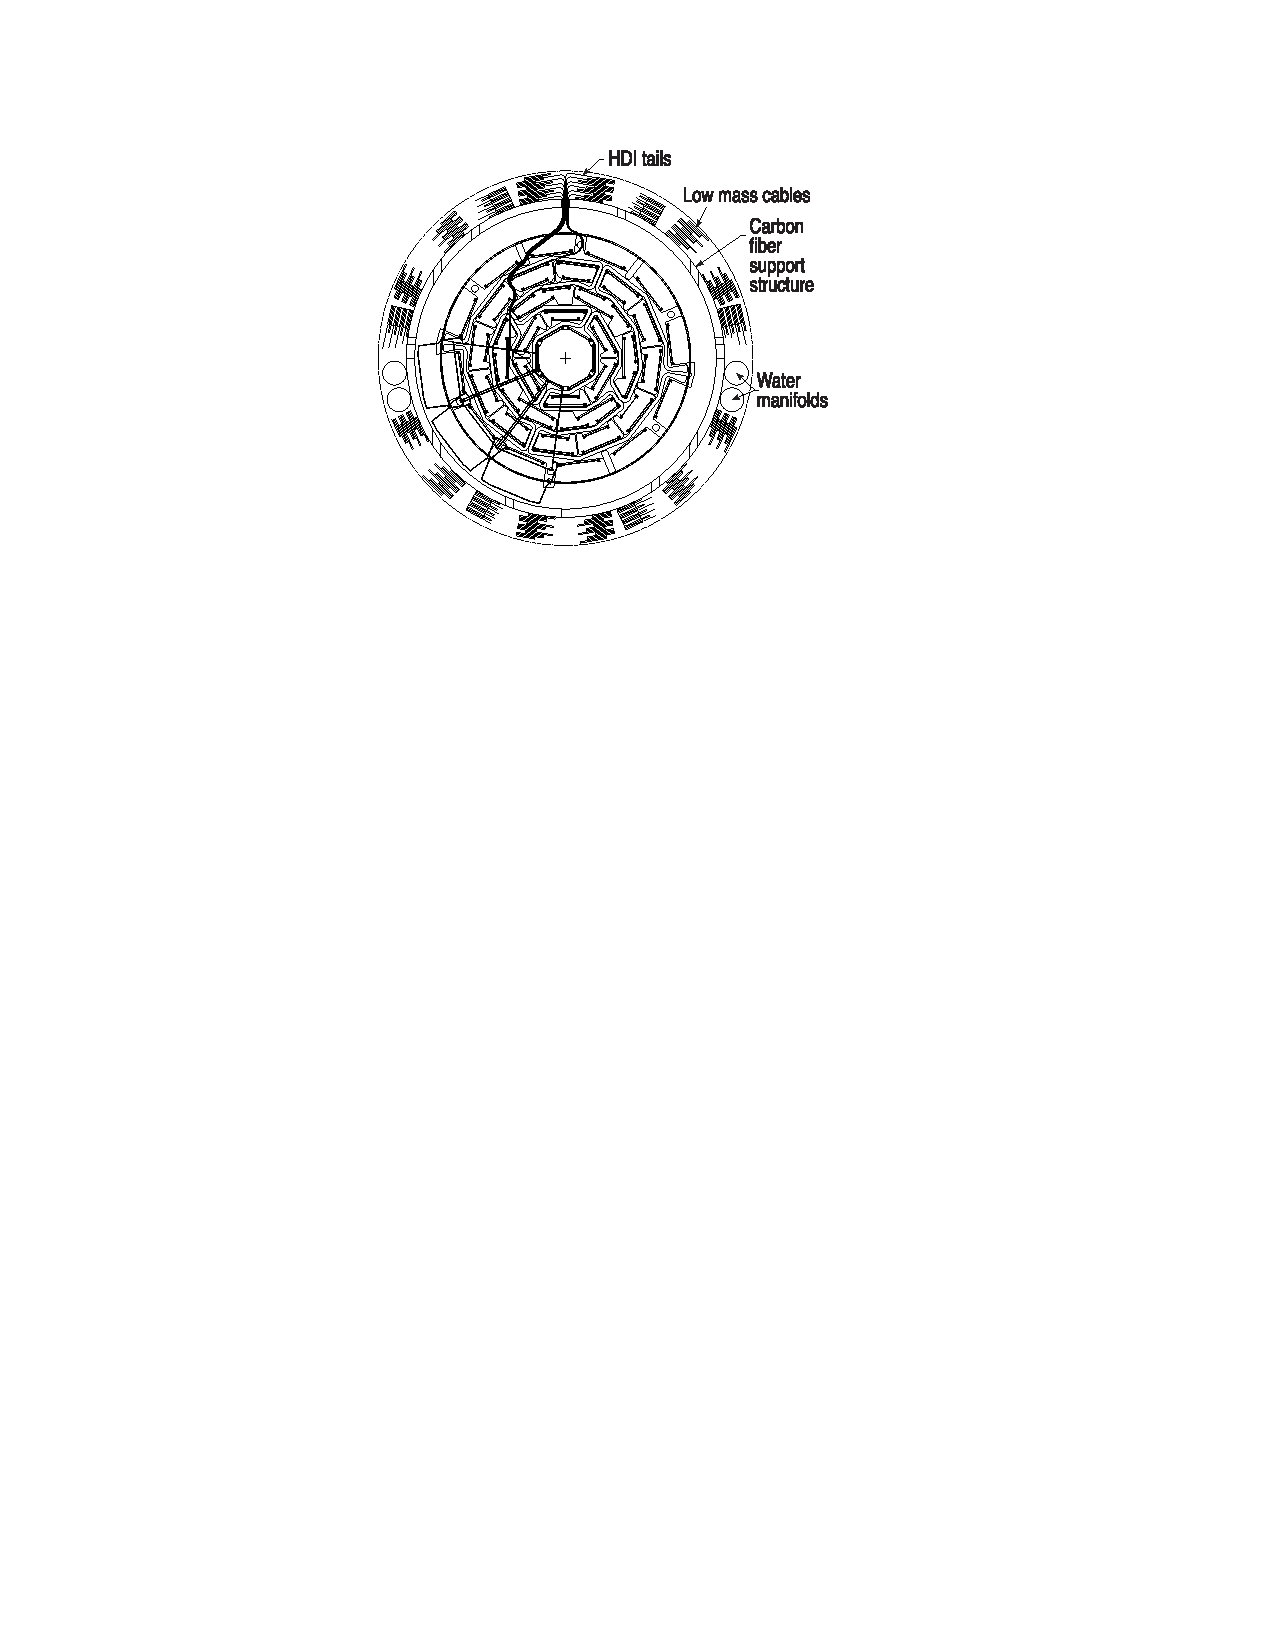
\includegraphics[height=0.6\textheight]{./Images/09_SMT_04}
      \caption*{{\scriptsize Cross section of the SMT disk/barrel module showing
            ladders mounted on the beryllium bulkhead, sample cable paths,
            three of twelve F-disk wedges, carbon fiber support structure,
            and the low-mass cable stack.}}
      \end{figure}
    % \itt
    % \item \textcolor{blue}{SMT support structure:\\}
    %   two double-walled carbon
    %   fiber cylinder.
    % \tti
\end{overlayarea}
\end{frame}


%%%%%%%% SLIDE
\begin{frame}{\textcolor{Goldenrod}{Silicon Microstrip Tracker Performance }}
  \begin{overlayarea}{\textwidth}{\textheight}
    \begin{figure}[h]
      \centering
      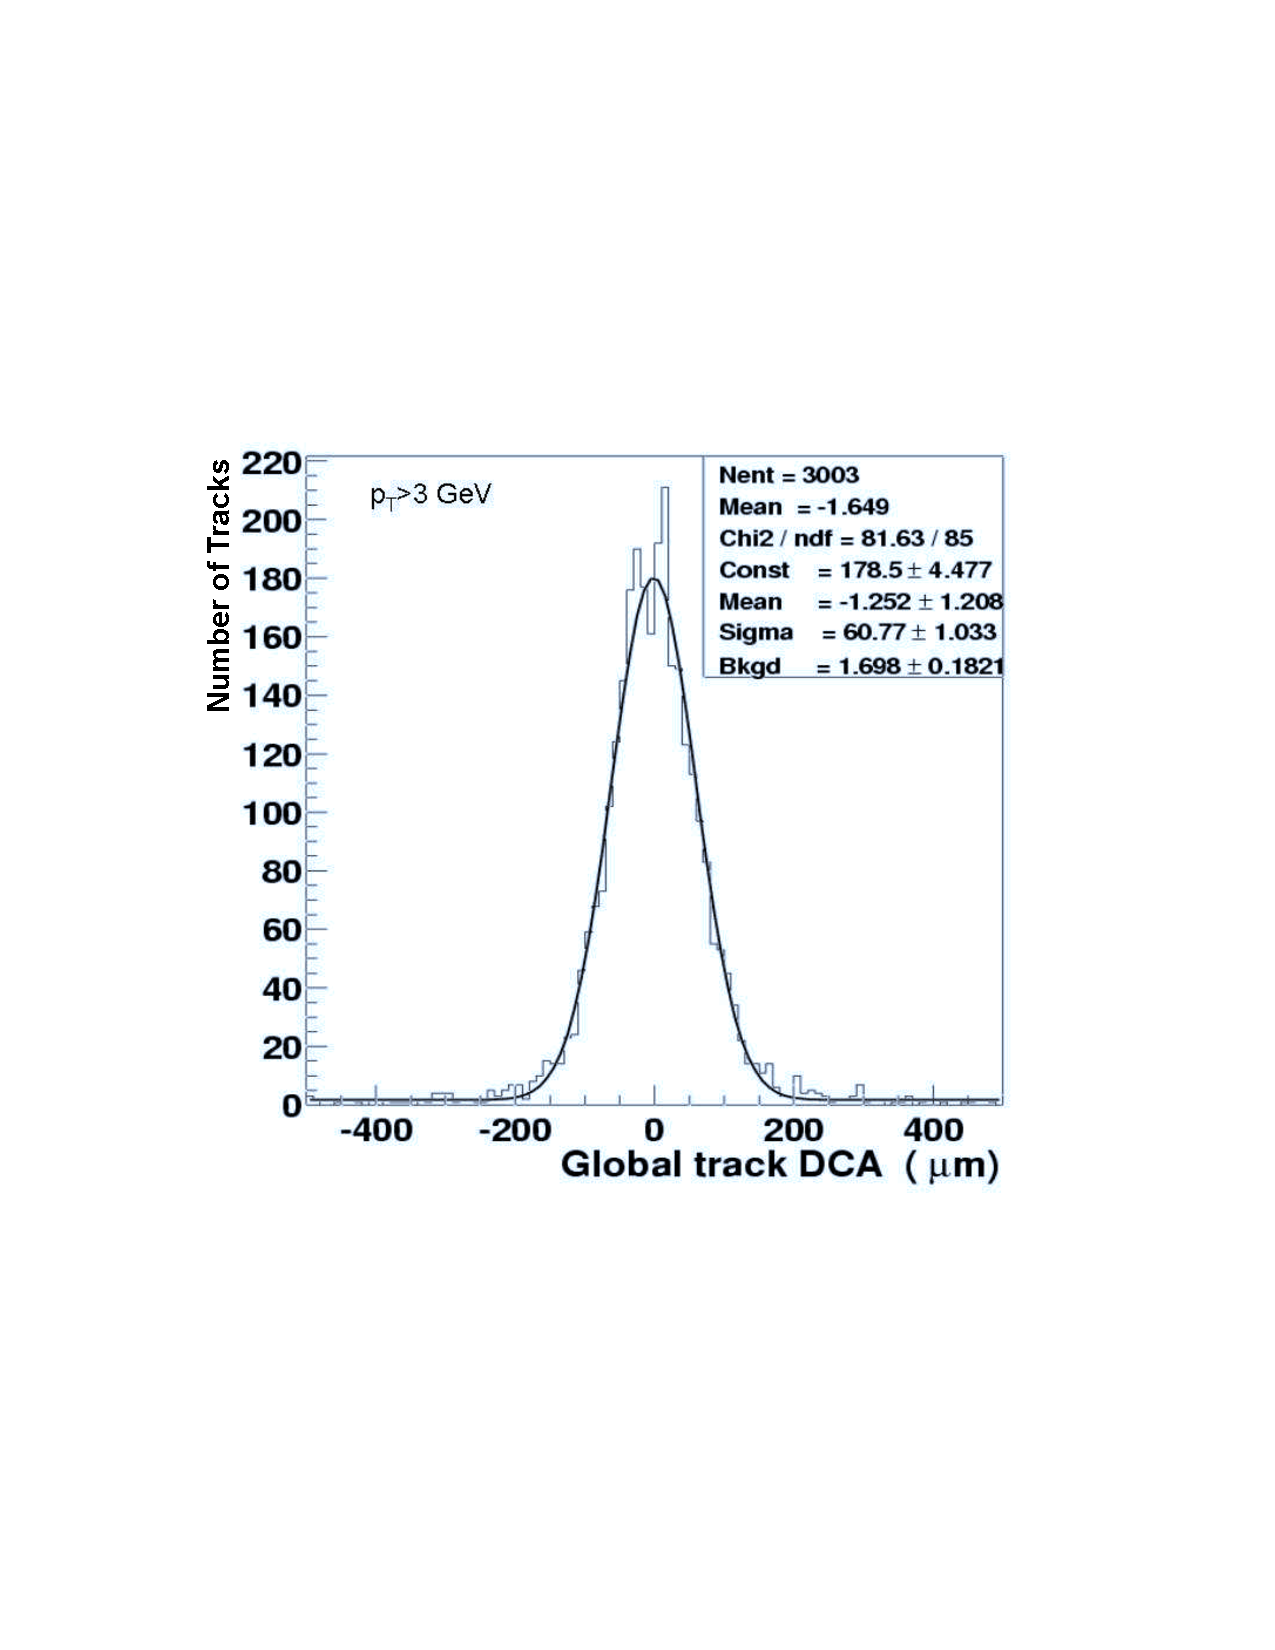
\includegraphics[height=0.45\textheight,width=0.4\textwidth]{./Images/11_SMT_01}
      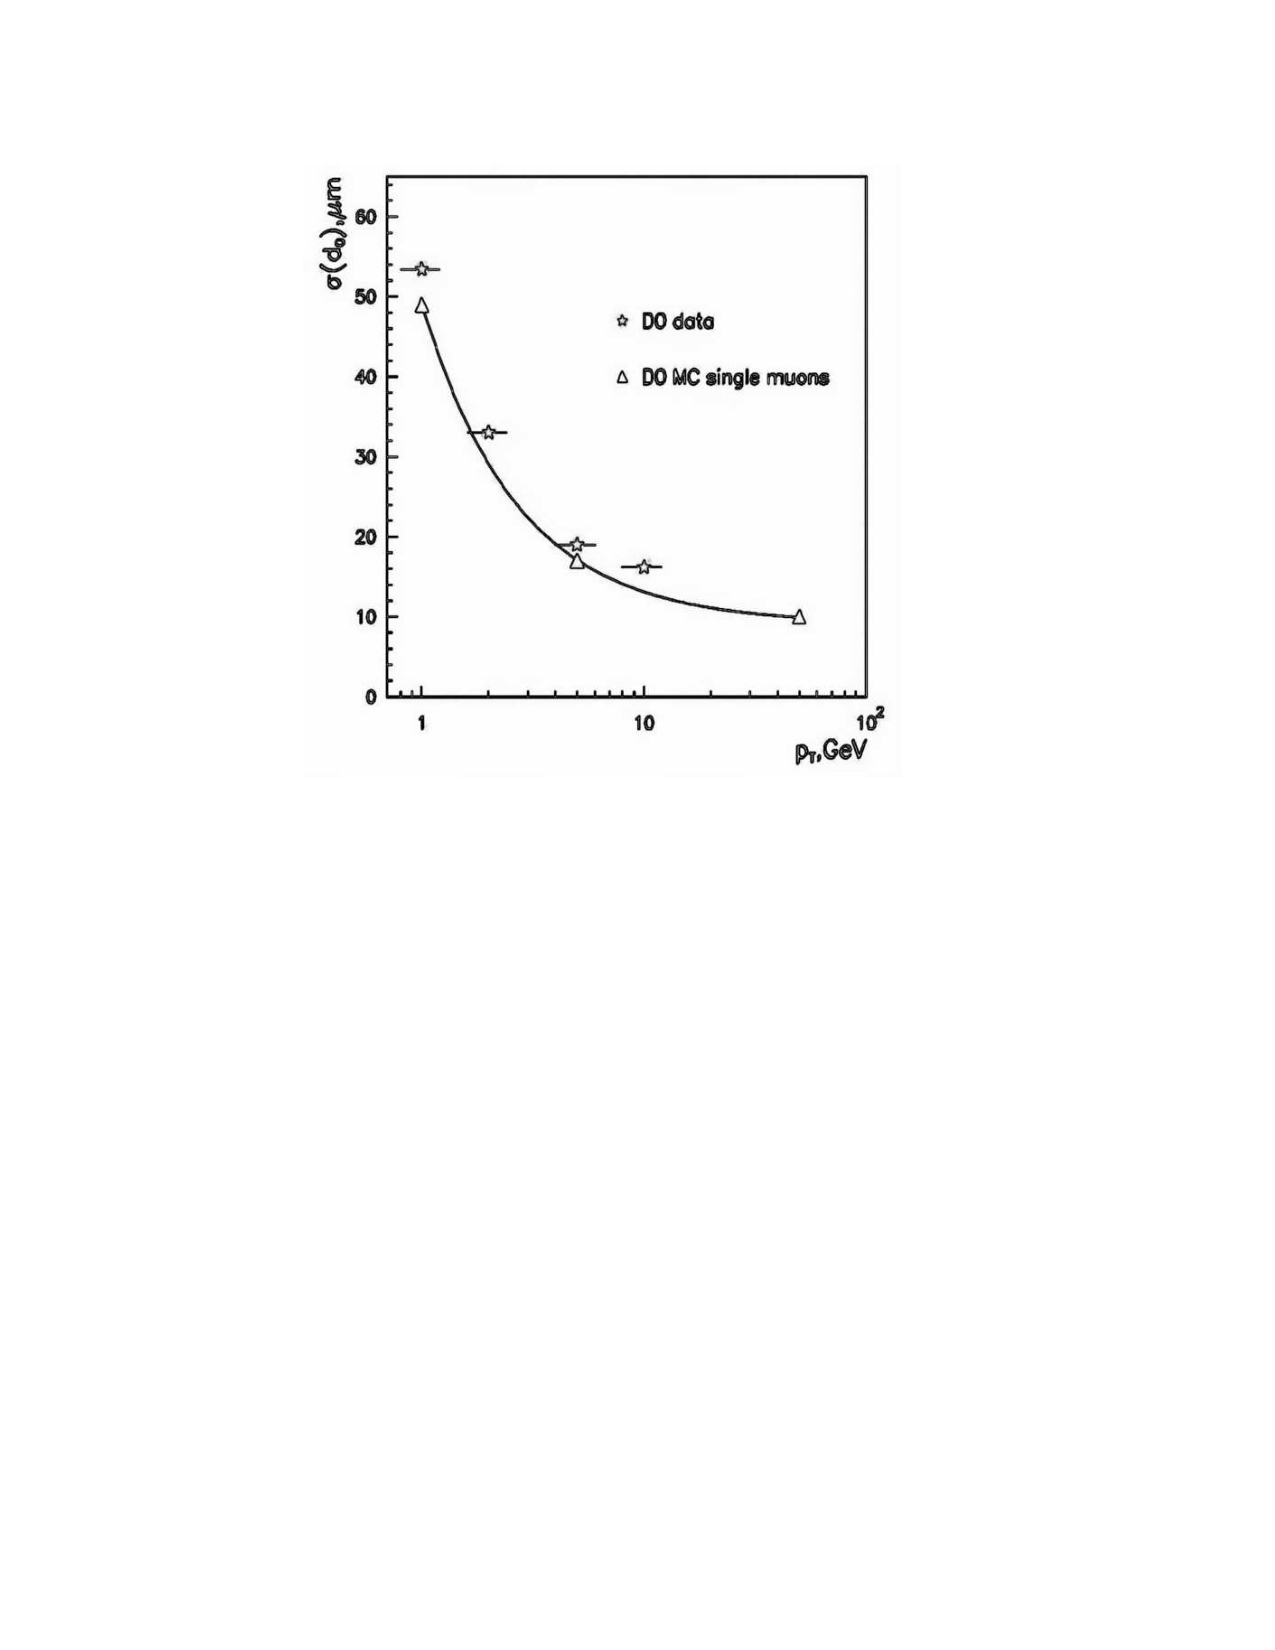
\includegraphics[height=0.45\textheight,width=0.4\textwidth]{./Images/12_SMT_01}
      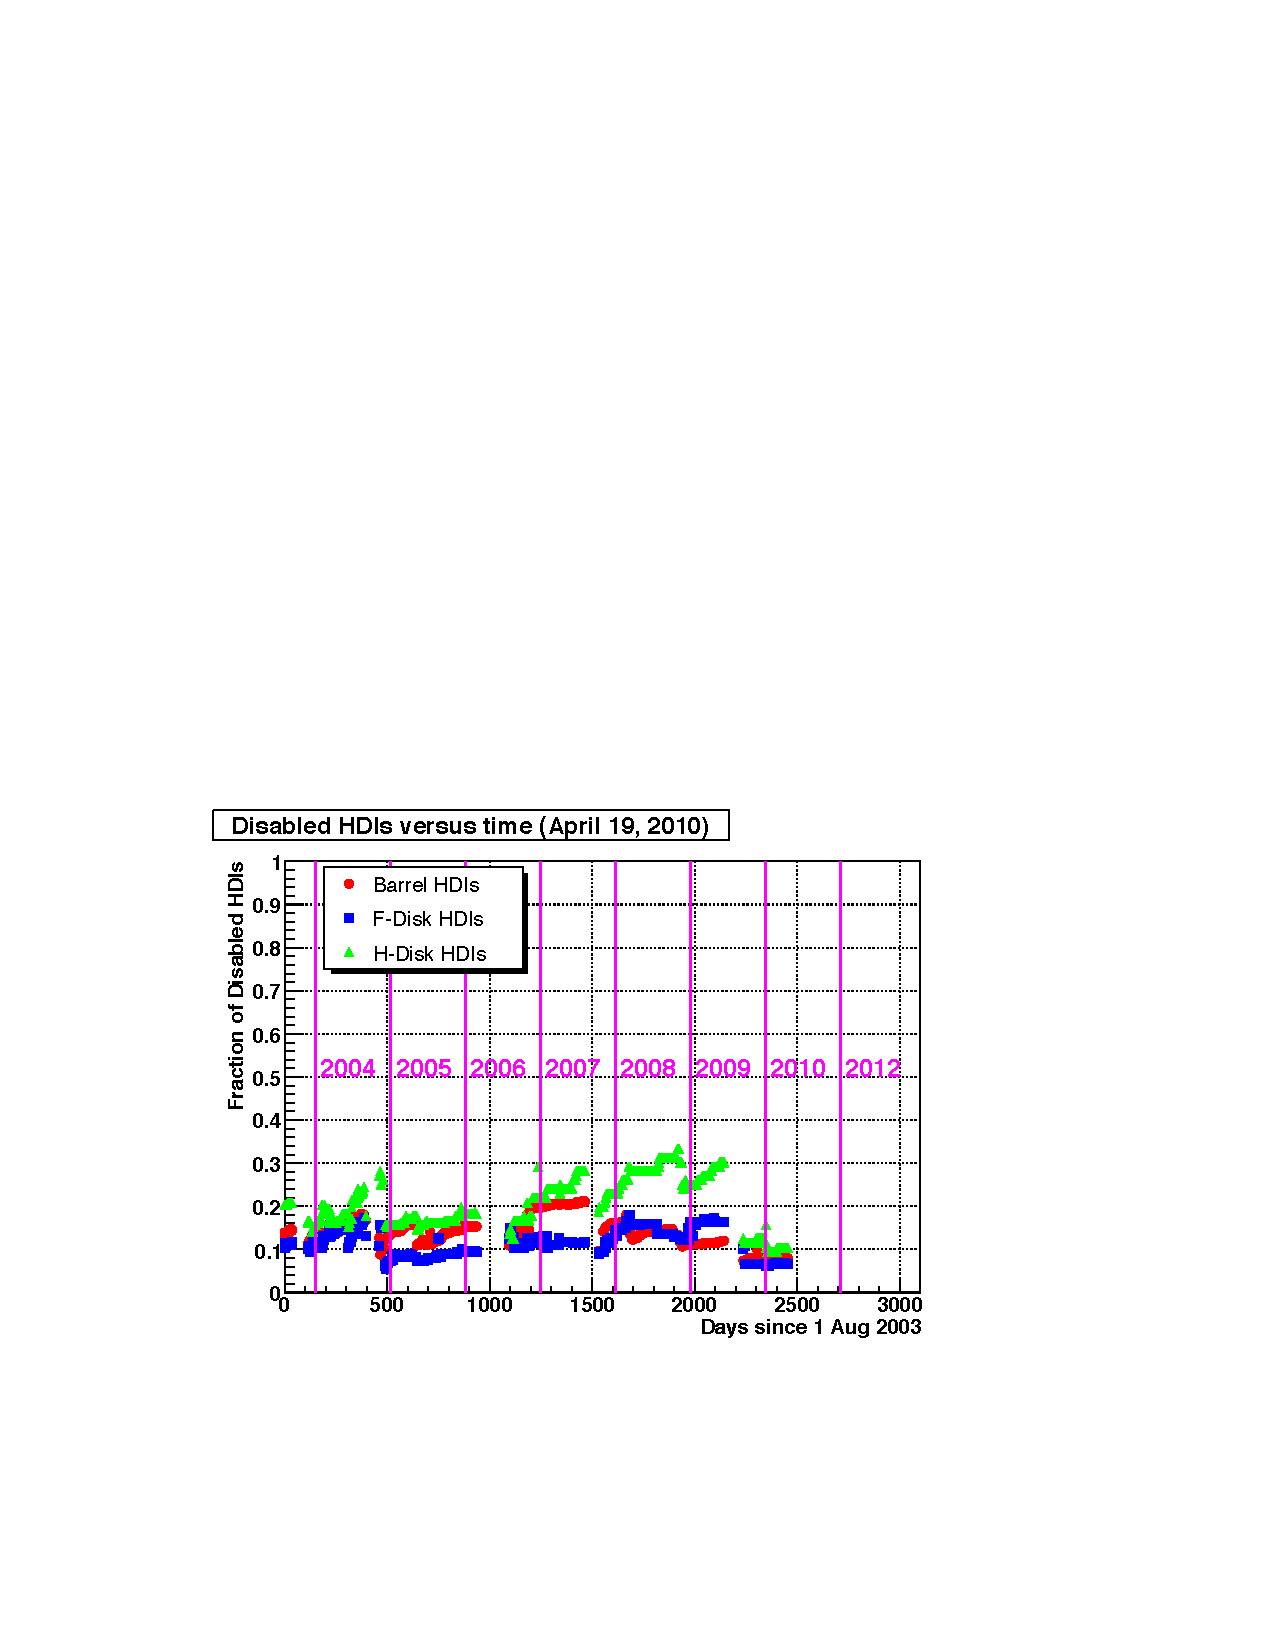
\includegraphics[height=0.45\textheight,width=0.3\textwidth]{./Images/12_SMT_02}
      
    \end{figure}
    \itt
  \item The signal/noise ratio is between $12-18$
    depending on the module type
    \note{The signal is defined as the cluster
      charge given by a minimum ionizing particle including a
      correction for the incident angle, and the noise as the rms of the
      pedestal distributions.}
  \item \alert{{\small $\sigma_{d_0} \approx 60 \mu m$ to which the beam size itself
        contributes $30$ to $40 \mu m$}}
    
  % \item \alert{using both the hits in the SMT and CFT $\to$ much better
  %     resolution $\sigma_{d_0} \approx 15 \mu m$}
  %   \tti
    
  % \item during run II $\approx 90$\% of sensors were functional
    \tti
\end{overlayarea}
\end{frame}

%%%%%%%% SLIDE
\begin{frame}{\textcolor{Goldenrod}{Silicon Microstrip Tracker Performance }}
  \(
  \<{0.5\textwidth}
  \img{12_SMT_03}\\
  {\scriptsize Axial residual distribution using tracks with $p_T > 3 GeV/c$}
  \>
  \<{0.6\textwidth}
  \itt
   \item[$a)$] upon
     initial installation and
   \item[$b)$] after software alignment of the central
     barrel detectors.
   \item the residual is the distance between the SMT hit
     and the track.
   \item \textcolor{blue}{the track fit was done using all SMT and CFT hits
       except the SMT hit in question.}
   \item \alert{the simulated resolution of the
     residual distribution for a perfectly aligned detector is about
     $16 \mu$.}
  \tti
  \>
  \)
\end{frame}


\subsection{Central fiber tracker}
%%%%%% SLIDE
\begin{frame}{\textcolor{Goldenrod}{Central Fiber Tracker}}
  \begin{overlayarea}{\textwidth}{\textheight}
    \begin{figure}[h]\centering
      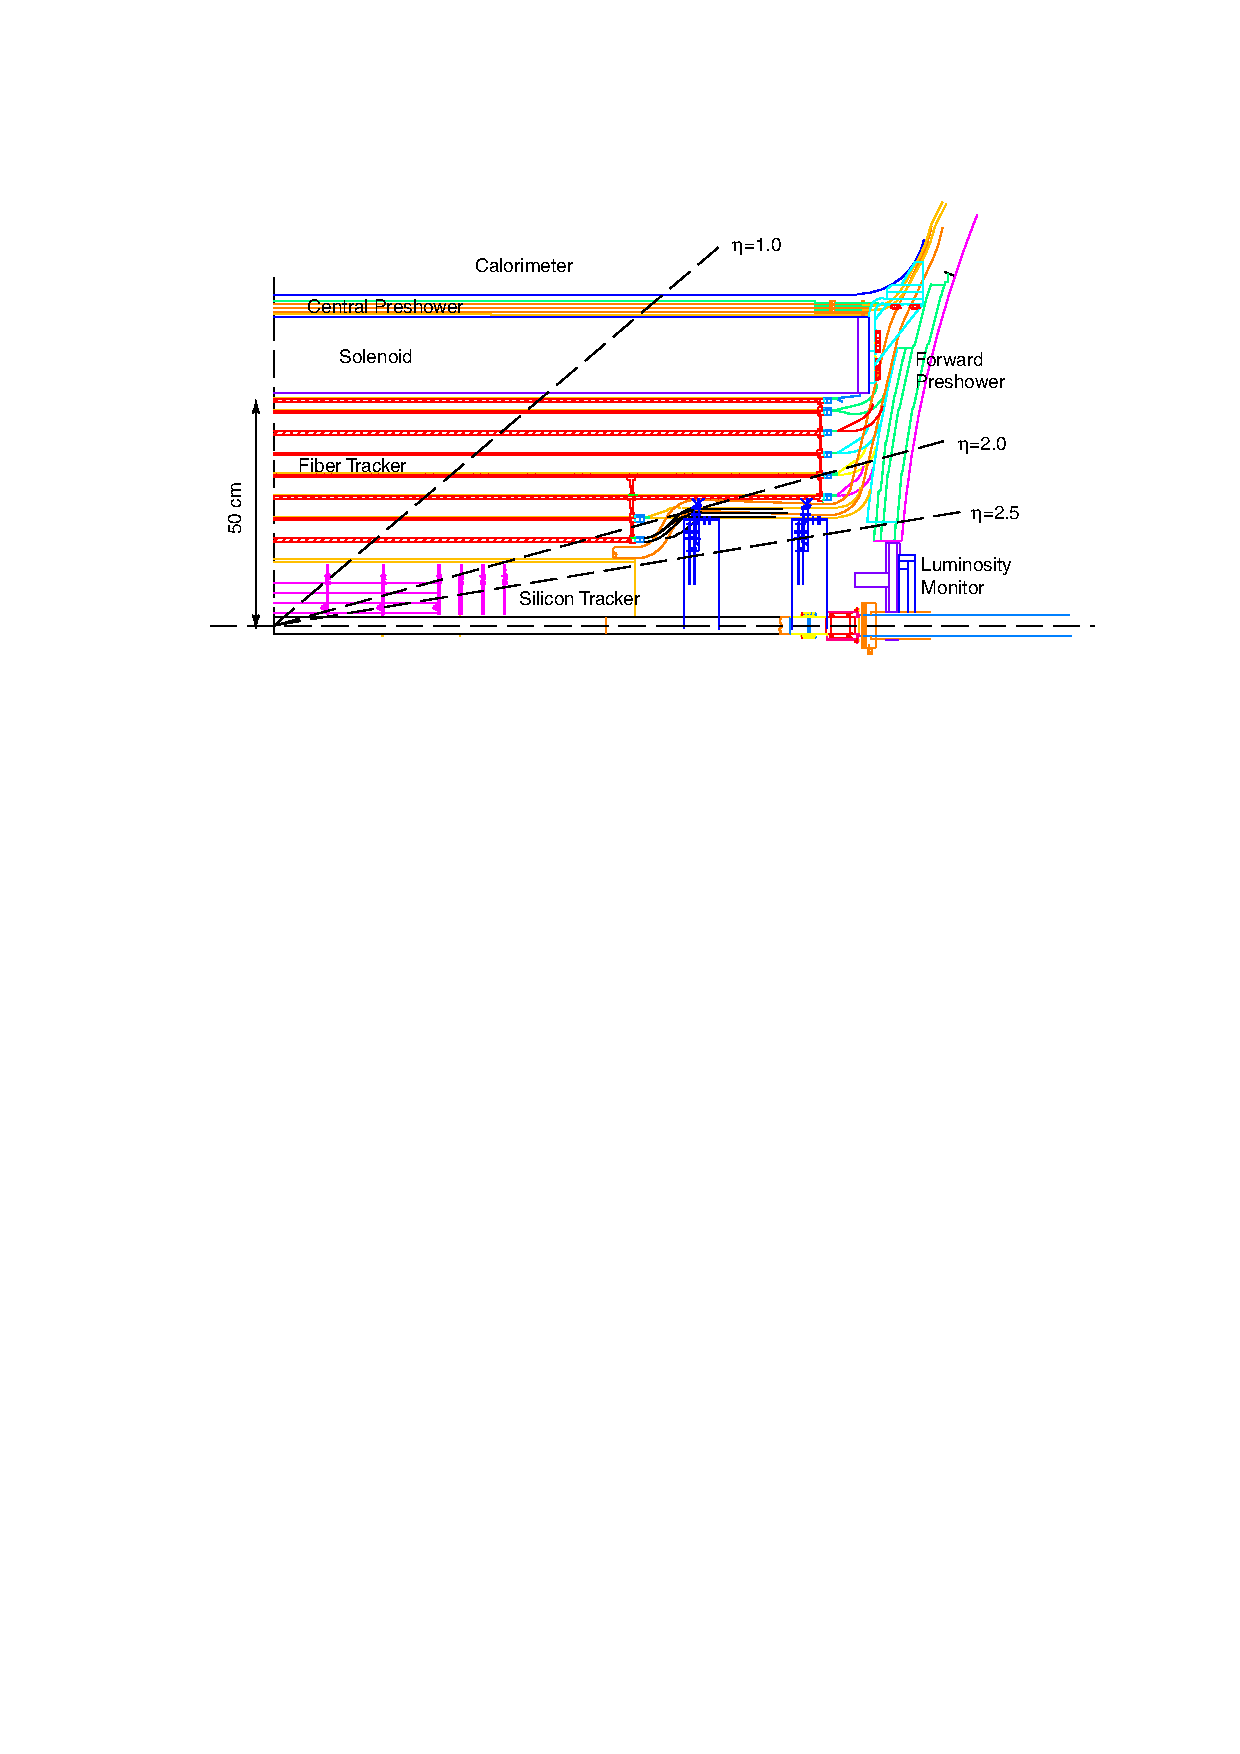
\includegraphics[height=0.4\textheight,width=0.7\textwidth]{./Images/08_CT_01.pdf}
      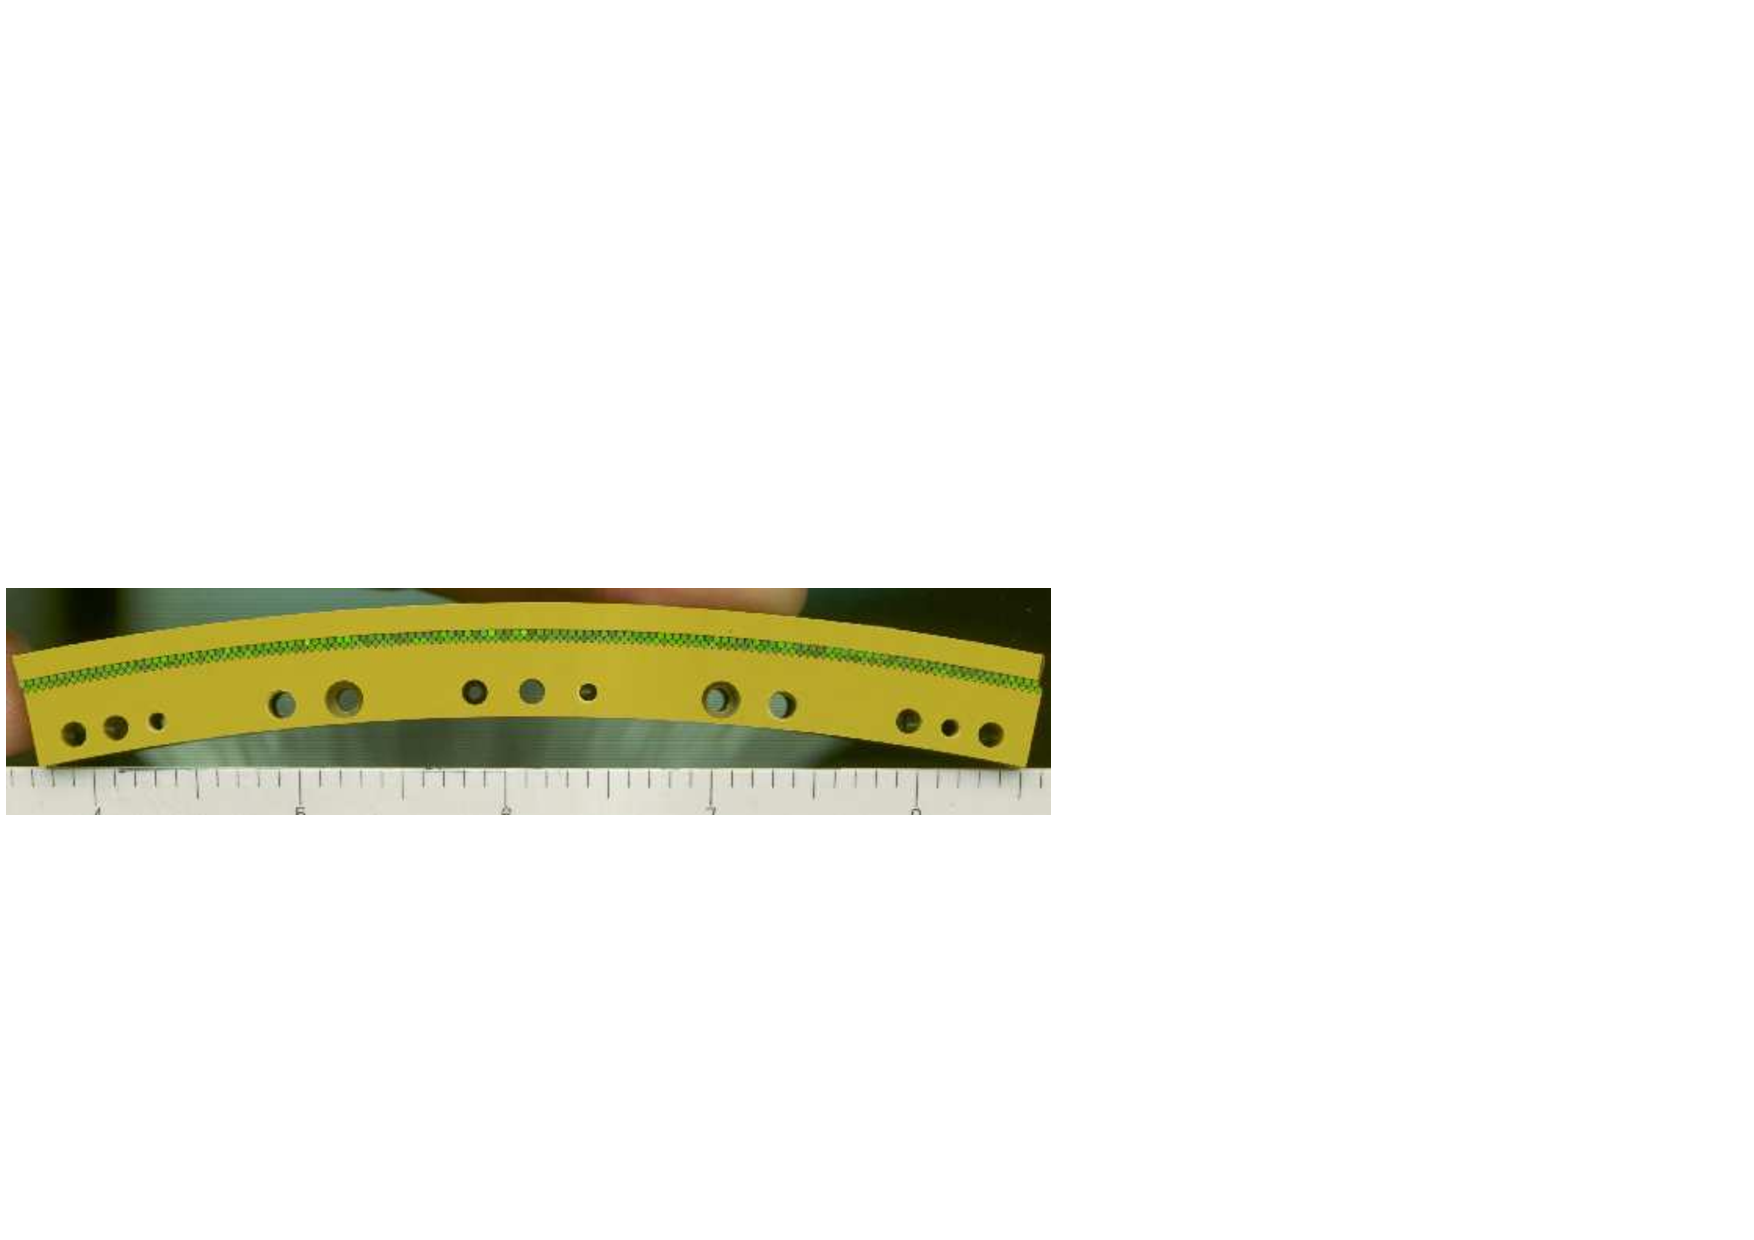
\includegraphics[height=0.2\textheight, width=0.3\textwidth]{./Images/15_CFT}
    \end{figure}
    \itt
    \note{scintillating fibers mounted on eight concentric
      support cylinders ($20 to 52 cm$ from
      the center of the beampipe. The
      two innermost cylinders are $1.66 m$ long; the outer six cylinders are
      $2.52 m$ long.}
    
    \note{ Each cylinder supports one doublet layer of fibers oriented
      along the beam direction and a second doublet layer at a
      stereo angle in $\phi$ of $+3^{\textdegree}$.}
    
  \item 8 coaxial carbon cylinders, each supporting 2 doublet layers
    of fibers in axial-u-v orientation ($3^{\textdegree}$)
  \item $76800$ fibers: made of polystyrene (PS), \it{paraterphenyl (PT) $1$\%, and
      3-hydroxyflavone (3HF)$0.15$\%}; $d = 835 \mu m ; l = 1.66/2.52 m$
    \tti
  \end{overlayarea}
\end{frame}

%%%%%% SLIDE
\begin{frame}{\textcolor{Goldenrod}{Central Fiber Tracker Light Collectors}}
  \(
  \<{0.3\textwidth}
  \img{21_CFT_VLPC.jpg}\\
  %\img{21_CFT_VLPC_01.jpg}\\
  \img{21_CFT_VLPC_02.jpg}\\
  \>
  \<{0.7\textwidth}
  \itt

  \item[$\bullet$] the fibres are connected by $7-11 m$ long optical waveguides to
    photodetectors positioned in a cryostat underneath the central
    calorimeter
  \item[$\bullet$] light collectors are Visible Light Photon Counters (VLPCs),
    (arsenic doped silicon diodes operating at temperatures
    of $10 K$)

  \item[$\bullet$] the VLPCs have quantum efficiencies of $\approx 80$\%, high gain and less
    than $0.1$\% average noise
  \item[$\bullet$] \alert{the axial fibre layers are used in the Level 1 trigger system}
  \tti
  \>
  \)
\end{frame}


%%%%%% SLIDE
\begin{frame}{\textcolor{Goldenrod}{Central Fiber Tracker: performance}}
  \begin{overlayarea}{\textwidth}{\textheight}
    \begin{figure}[h]\centering
      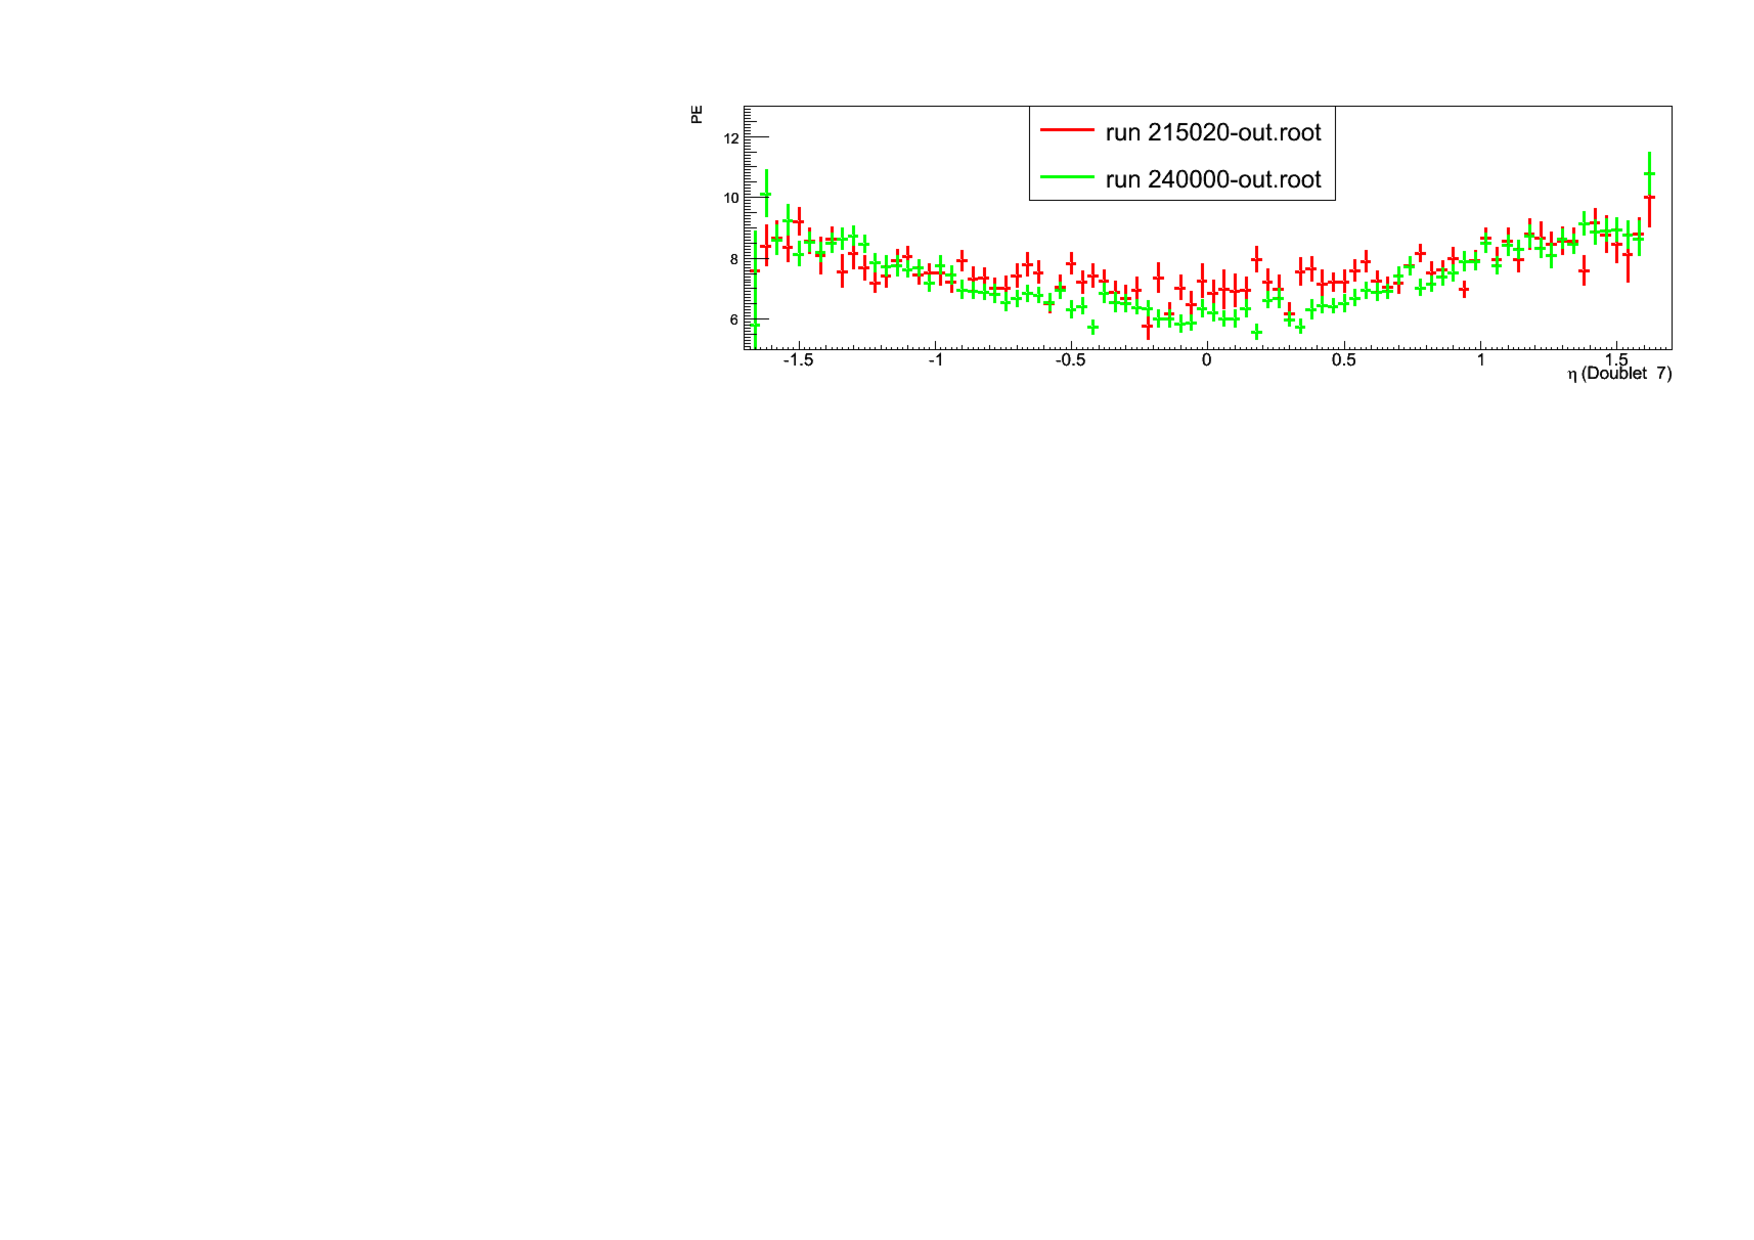
\includegraphics[height=0.2\textheight]{./Images/22_CFT_performance.pdf}\\
      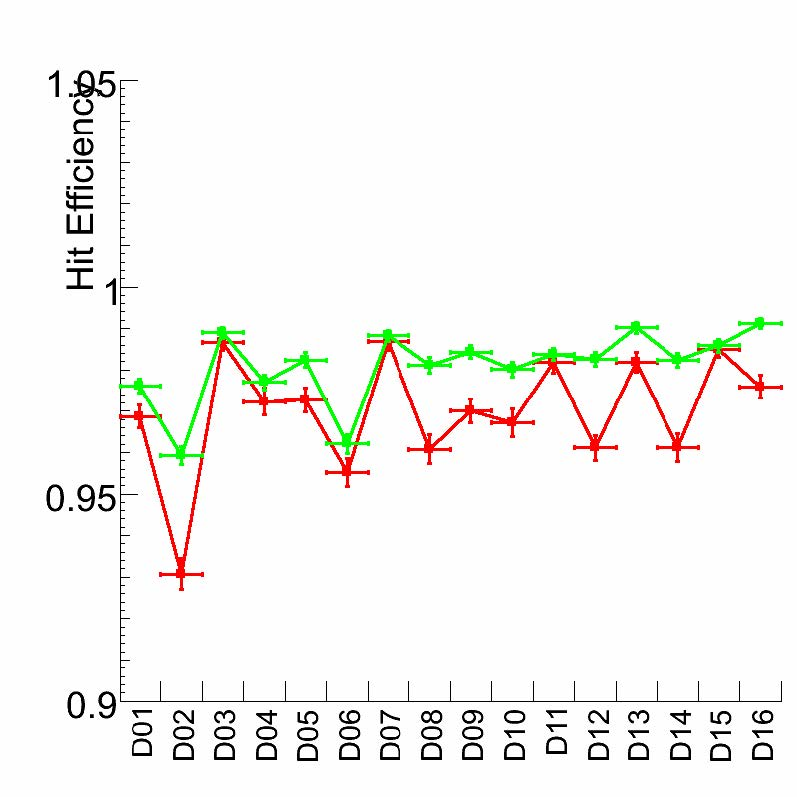
\includegraphics[height=0.45\textheight]{./Images/23_CFT_performance}
      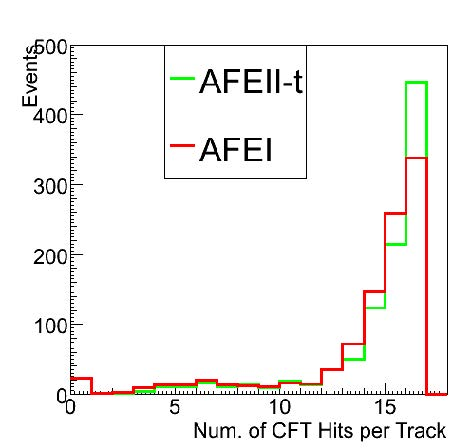
\includegraphics[height=0.45\textheight]{./Images/24_CFT_performance}
      \caption*{{\scriptsize average photon yield, hit efficiency, and number of CFT
          hits per track}}
    \end{figure}
 \end{overlayarea}
\end{frame}

% %%%%%% SLIDE
% \begin{frame}{\textcolor{Goldenrod}{Central Fiber Tracker: Central Track Tigger (CTT)}}
%   \(
%   \<{0.7\textwidth}
%   \itt[<+->]
% \item Counts track candidates identified in axial view of CFT by
%   looking for hits in all 8 axial layers
% \item Combines tracking and preshower information to identify
%   electron and photon candidates
% \item
%   Generates track lists allowing other trigger systems to
%   perform track matching
%   \tti
%   \>
%   \<{0.3\textwidth}
%   \img{20_CFT}
%   \>
%   \)
% \end{frame}

